\documentclass[letterpaper,10pt]{article}

\usepackage{enumitem}
\usepackage{titling}
\usepackage{listings,listings-rust}
\usepackage{url}
\usepackage{soul}
\usepackage{hyperref}
\usepackage{setspace}
\usepackage{subfig}
\usepackage{sectsty}
\usepackage{pdfpages}
\usepackage{colortbl}
\usepackage{multirow}
\usepackage{multicol}
\usepackage{relsize}
\usepackage{amsmath}
\usepackage{wasysym}
\usepackage{fancyvrb}
\usepackage[yyyymmdd]{datetime}
\usepackage{amsmath,amssymb,amsthm,graphicx,xspace}
\usepackage[titlenotnumbered,noend,noline]{algorithm2e}
\usepackage[compact]{titlesec}
\usepackage{XCharter}
\usepackage[T1]{fontenc}
\usepackage[scaled]{beramono}
\usepackage[normalem]{ulem}
\usepackage{booktabs}
\usepackage{tikz}
\usetikzlibrary{arrows.meta,automata,shapes,trees,matrix,chains,scopes,positioning,calc,decorations.pathreplacing}
\tikzstyle{block} = [rectangle, draw, fill=blue!20, 
    text width=2.5em, text centered, rounded corners, minimum height=2em]
\tikzstyle{bw} = [rectangle, draw, fill=blue!20, 
    text width=4em, text centered, rounded corners, minimum height=2em]

\definecolor{namerow}{cmyk}{.40,.40,.40,.40}
\definecolor{namecol}{cmyk}{.40,.40,.40,.40}
\renewcommand{\dateseparator}{-}

\let\LaTeXtitle\title
\renewcommand{\title}[1]{\LaTeXtitle{\textsf{#1}}}

\lstset{basicstyle=\footnotesize\ttfamily,breaklines=true}

\newcommand{\CPP}{C\nolinebreak\hspace{-.05em}\raisebox{.4ex}{\tiny\bf +}\nolinebreak\hspace{-.10em}\raisebox{.4ex}{\tiny\bf +}}
\def\CPP{{C\nolinebreak[4]\hspace{-.05em}\raisebox{.4ex}{\tiny\bf ++}}}

\newcommand{\handout}[5]{
  \noindent
  \begin{center}
  \framebox{
    \vbox{
      \hbox to 5.78in { {\bf ECE459: Programming for Performance } \hfill #2 }
      \vspace{4mm}
      \hbox to 5.78in { {\Large \hfill #4  \hfill} }
      \vspace{2mm}
      \hbox to 5.78in { {\em #3 \hfill \today} }
    }
  }
  \end{center}
  \vspace*{4mm}
}

\newcommand{\lecture}[3]{\handout{#1}{#2}{#3}{Lecture#1}}
\newcommand{\tuple}[1]{\ensuremath{\left\langle #1 \right\rangle}\xspace}

\addtolength{\oddsidemargin}{-1.000in}
\addtolength{\evensidemargin}{-0.500in}
\addtolength{\textwidth}{2.0in}
\addtolength{\topmargin}{-1.000in}
\addtolength{\textheight}{1.75in}
\addtolength{\parskip}{\baselineskip}
\setlength{\parindent}{0in}
\renewcommand{\baselinestretch}{1.5}
\newcommand{\term}{Winter 2020}

\singlespace


\begin{document}

\lecture{8 --- Asynchronous I/O, epoll, select}{\term}{Patrick Lam}

\section*{Asynchronous/non-blocking I/O}

Let's start with some juicy quotes.

\begin{center}
  \fbox{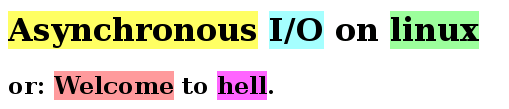
\includegraphics[width=.7\textwidth]{images/aio-linux.png}}\\
{\scriptsize (mirrored at \url{compgeom.com/~piyush/teach/4531_06/project/hell.html})}
   \\[2em]

   ``Asynchronous I/O, for example, is often infuriating.''\\
\hfill --- Robert Love. {\em Linux System Programming, 2nd ed, } page 215.

\end{center}

To motivate the need for non-blocking I/O, consider some standard I/O code:

\begin{verbatim}
    fd = open(...);
    read(...);
    close(fd);
\end{verbatim}

This isn't very performant. The problem is that the {\tt read} call will
{\em block}. So, your program doesn't get to use the zillions of CPU cycles that
are happening while the I/O operation is occurring.

\paragraph{As seen previously: threads.} That can be fine if
you have some other code running to do work---for instance, other threads
do a good job mitigating the I/O latency, perhaps doing I/O themselves.
But maybe you would rather not use threads. Why not?

\begin{itemize}
\item potential race conditions;
\item overhead due to per-thread stacks; or
\item limitations due to maximum numbers of threads.
\end{itemize}

\paragraph{Live coding example.} To illustrate the max-threads
issue, let's write {\tt threadbomb.c}, to explore how many simultaneous threads
one could start on my computer.

\paragraph{Non-blocking I/O.} The main point of this lecture, though,
is non-blocking/asynchronous I/O. The simplest example:

\begin{verbatim}
    fd = open(..., O_NONBLOCK);
    read(...); // returns instantly!
    close(fd);
\end{verbatim}

In principle, the {\tt read} call is supposed to return instantly,
whether or not results are ready. That was easy!

Well, not so much. The {\tt O\_NONBLOCK} flag actually only has the
desired behaviour on sockets. The semantics of {\tt O\_NONBLOCK} is
for I/O calls to not block, in the sense that they should never wait
for data while there is no data available.

Unfortunately, files always have data available. Under Linux, you'd have
to use {\tt aio} calls to be able to send requests to the I/O subsystem
asynchronously and not, for instance, wait for the disk to spin up.
We won't talk about them, but they operate along the same lines as what
we will see. They just have a different API.

\paragraph{Conceptual view: non-blocking I/O.} Fundamentally,
there are two ways to find out whether I/O is ready to be queried:
polling (under UNIX, implemented via {\tt select}, {\tt poll},
and {\tt epoll}) and interrupts (under UNIX, signals).


We will describe {\tt epoll}. It is the most modern and
flexible interface. Unfortunately, I didn't realize that the obvious
{\tt curl} interface does not work with {\tt epoll} but instead with
{\tt select}.  There is different syntax but the ideas are the same.

The key idea is to give {\tt epoll} a bunch of file descriptors and
wait for events to happen. In particular:
     \begin{itemize}
       \item create an epoll instance ({\tt epoll\_create1});
       \item populate it with file descriptors ({\tt epoll\_ctl}); and
       \item wait for events ({\tt epoll\_wait}).
     \end{itemize}
Let's run through these steps in order.

\paragraph{Creating an {\tt epoll} instance.} Just use the API:
    \begin{verbatim}
   int epfd = epoll_create1(0);
    \end{verbatim}

The return value {\tt epfd} is typed like a UNIX file
descriptor---{\tt int}---but doesn't represent any files; instead, use
it as an identifier, to talk to {\tt epoll}.

The parameter ``{\tt 0}'' represents the flags, but the only available flag
is {\tt EPOLL\_CLOEXEC}. Not interesting to you.

\paragraph{Populating the {\tt epoll} instance.} Next, you'll want
{\tt epfd} to do something. The obvious thing is to add some {\tt fd}
to the set of descriptors watched by {\tt epfd}:
    \begin{verbatim}
   struct epoll_event event;
   int ret;
   event.data.fd = fd;
   event.events = EPOLLIN | EPOLLOUT;
   ret = epoll_ctl(epfd, EPOLL_CTL_ADD, fd, &event);
    \end{verbatim}

You can also use {\tt epoll\_ctl} to modify and delete descriptors from {\tt epfd}; read the manpage to find out how.

\paragraph{Waiting on an {\tt epoll} instance.} Having completed
the setup, we're ready to wait for events on any file descriptor in {\tt epfd}.
    \begin{verbatim}
  #define MAX_EVENTS 64

  struct epoll_event events[MAX_EVENTS];
  int nr_events;

  nr_events = epoll_wait(epfd, events, MAX_EVENTS, -1);
    \end{verbatim}

The given {\tt -1} parameter means to wait potentially forever;
otherwise, the parameter indicates the number of milliseconds to wait.
(It is therefore ``easy'' to sleep for some number of milliseconds by
starting an {\tt epfd} and using {\tt epoll\_wait}; takes two function
calls instead of one, but allows sub-second latency.)

Upon return from {\tt epoll\_wait}, we know that we have {\tt
  nr\_events} events ready.

\subsection*{Level-Triggered and Edge-Triggered Events}
One relevant concept for these polling APIs is the concept of
\emph{level-triggered} versus \emph{edge-triggered}.  The default {\tt
  epoll} behavious is level-triggered: it returns whenever data is
ready. One can also specify (via {\tt epoll\_ctl}) edge-triggered
behaviour: return whenever there is a change in readiness.

%\paragraph{Another Live Demo.} Now let's run some code (socket.c) that creates a
%server and reads from it, in either level-triggered mode or edge-triggered mode.

One would think that level-triggered mode would return from {\tt read}
whenever data was available, while edge-triggered mode would return
from {\tt read} whenever new data came in. Level-triggered does behave
as one would guess: if there is data available, {\tt read()} returns
the data. However, edge-triggered mode returns whenever the
state-of-readiness of the socket changes (from no-data-available to
data-available). Play with it and get a sense for how it works.

Good question to think about: when is it appropriate to choose one or the other?

\subsection*{Asynchronous I/O}
As mentioned above, the POSIX standard defines {\tt aio} calls.
Unlike just giving the {\tt O\_NONBLOCK} flag, using {\tt aio} works
for disk as well as sockets.

\paragraph{Key idea.} You specify the action to occur when I/O is ready:
    \begin{itemize}
      \item nothing;
      \item start a new thread; or
      \item raise a signal.
    \end{itemize}

Your code submits the requests using e.g. {\tt aio\_read} and {\tt aio\_write}.
If needed, wait for I/O to happen using {\tt aio\_suspend}.

\paragraph{Nonblocking I/O with curl.} The next lecture notes give more clue
about nonblocking I/O with curl. Although it doesn't work with {\tt epoll}
but rather {\tt select}, it uses the same ideas---we'll therefore see two
(three, with aio) different implementations of the same idea. 
Briefly, you:
\begin{itemize}
\item build up a set of descriptors;
\item invoke the transfers and wait for them to finish; and
\item see how things went.
\end{itemize}

\section*{curl\_multi}
It's important to see at least one specific example of an idea. I talked about
{\tt epoll} and I meant that to be the specific example, but we 
can't quite use it without getting into socket programming, and I don't want to
do that. Instead, we'll see non-blocking I/O in the specific example of the curl
library, which is reasonably widely used in the Linux world.

Tragically, it's complicated to use {\tt epoll} with {\tt curl\_multi}, and I couldn't
quite figure it out. So I'll describe the {\tt select}-based interface for {\tt curl\_multi}.
A socket-based interface which works with {\tt epoll} also exists. I won't talk about that.

The relevant steps, in any case, are:
\begin{itemize}
\item Create individual requests with {\tt curl\_easy\_init}.
\item Create a multi-handle with {\tt curl\_multi\_init} and add the requests to it
with {\tt curl\_multi\_add\_handle}.
\item (for select-based interface:) put in requests \& wait for results, using {\tt 
curl\_multi\_perform}. That call generalizes {\tt curl\_easy\_perform}.
\item Handle completed transfers with {\tt curl\_multi\_info\_read}.
\end{itemize}

\paragraph{On the use of {\tt curl\_multi\_perform}.} The actual non-blocking read/write
is done in {\tt curl\_multi\_perform}, which returns the number of still-active handles 
through its parameter.

You call it in a loop, with a call to {\tt select} above. Call {\tt select} and then
{\tt curl\_multi\_perform} in a loop while there are still running transfers.
You're also allowed to manipulate (delete/alter/re-add) a {\tt curl\_easy\_handle} whenever
a transfer finishes.

\paragraph{Setting up the {\tt select}.} Before you call {\tt curl\_multi\_perform}
and {\tt select}, you need to set up the {\tt select}. The curl call {\tt curl\_multi\_fdset}
sets up the parameters for the {\tt select}, while {\tt curl\_multi\_timeout} gives you
the proper timeout to hand to {\tt select}.

\begin{verbatim}
    // zero the fd-sets
    FD_ZERO(&fdread); FD_ZERO(&fdwrite); FD_ZERO(&fdexcep);
    // retrieve the fds, check for error
    curl_multi_fdset(multi_handle, 
                     &fdread, &fdwrite, &fdexcep, &maxfd);
    if (maxfd < -1) abort_("multi_fdset: couldn't wait for fds");
    // retrieve the timeout
    curl_multi_timeout(multi_handle, &curl_timeout);
\end{verbatim}

In an API infelicity, you have to convert the {\tt curl\_timeout} into a
{\tt struct timeval} for use by {\tt select}.

\paragraph{Calling {\tt select}.}
The call itself is fairly straightforward:
\begin{verbatim}
  rc = select(maxfd + 1, &fdread, &fdwrite, &fdexcep, &timeout);
  if (rc == -1) abort_("[main] select error");
\end{verbatim}
This waits for one of the file descriptors to become ready, or for the
timeout to elapse (whichever happens first).

Of course, once {\tt select} returns, you only know that something
happened, but you haven't done the work yet. So you then need to call
{\tt curl\_multi\_perform} again to do the work.

Finally, you get the results of {\tt curl\_multi\_perform} by calling
{\tt curl\_multi\_info\_read}. It also tells you how many messages are left.
\begin{verbatim}
  msg = curl_multi_info_read(multi_handle, &msgs_left);
\end{verbatim}
The return value \verb+msg->msg+ can be either {\tt CURLMSG\_DONE} or an error.
The handle \verb+msg->easy_handle+ tells you which handle finished. You may have
to look that up in your collection of handles.

Some gotchas (thanks Desiye Collier):
\begin{itemize}
\item Checking \verb+msg->msg == CURLMSG_DONE+ is not sufficient to ensure that a curl request actually happened. You also need to check {\tt data.result}.
\item (A1 hint:) To reset an individual handle in the {\tt multi\_handle}, you need to ``replace'' it. But you shouldn't use {\tt curl\_easy\_init()} to replace the handle.  In fact, you don't need a new handle at all.
\end{itemize}

\paragraph{Cleanup.} Always clean up after yourself! Use {\tt curl\_multi\_cleanup}
to destroy the multi-handle and {\tt curl\_easy\_cleanup} to destroy each individual handle. If you replace the {\tt curl\_easy\_init} call by {\tt curl\_global\_init} for the multithreaded case (which is a good idea), then you should use {\tt curl\_global\_cleanup} to clean up.

\paragraph{Example.}
There is a not-great example at 
\begin{center}
\url{http://curl.haxx.se/libcurl/c/multi-app.html}
\end{center}
but I'm not even sure it works verbatim. You could use it as a solution template,
but you'll need to add more code---I asked you to replace completed transfers in the
{\tt curl\_multi}.

\paragraph{A better way to use sockets.} Late-breaking news: instead
of that {\tt select()} crud, use {\tt curl\_multi\_wait()}, which is
just better, and easy to use. An example:
\url{https://gist.github.com/clemensg/4960504}

\paragraph{About that socket-based alternative.} There is yet another interface which
would allow you to use {\tt epoll}, but I couldn't figure it out. Sorry. The advantage,
beyond using {\tt epoll}, is that {\tt libcurl} doesn't need to scan over all of the transfers
when it receives notice that a transfer is ready. This can help when there are lots of sockets
open.

From the manpage:
\begin{itemize}
\item Create a multi handle

\item Set the socket callback with {\tt CURLMOPT\_SOCKETFUNCTION}

\item Set the timeout callback with {\tt CURLMOPT\_TIMERFUNCTION}, to get to know what timeout value to use when waiting for socket activities.

\item Add easy handles with {\tt curl\_multi\_add\_handle()}

\item Provide some means to manage the sockets libcurl is using, so you can check them for activity. This can be done through your application code, or by way of an external library such as libevent or glib.

\item Call {\tt curl\_multi\_socket\_action(..., CURL\_SOCKET\_TIMEOUT, 0, ...)} to kickstart everything. To get one or more callbacks called.

\item Wait for activity on any of libcurl's sockets, use the timeout value your callback has been told.

\item When activity is detected, call {\tt curl\_multi\_socket\_action()} for the socket(s) that got action. If no activity is detected and the timeout expires, call {\tt curl\_multi\_socket\_action(3)} with {\tt CURL\_SOCKET\_TIMEOUT}. 
\end{itemize}
There's an example, which has too many moving parts, here:
\begin{center}
\url{http://curl.haxx.se/libcurl/c/hiperfifo.html}
\end{center}
It uses {\tt libevent}, which I totally don't want to talk about in this class.

\section*{Building Servers: Concurrent Socket I/O}
Switching gears, we'll talk about building software that handles tons of connections. Let's go back to that initial question:

    \begin{quote}
      What is the ideal design for server process in Linux that handles concurrent socket I/O?
    \end{quote}

    So far in this class, we've seen:
    \begin{itemize}
    \item processes;
    \item threads; 
    \item thread pools; and
    \item non-blocking/async I/O.
    \end{itemize}

We'll analyze the answer by Robert Love, Linux kernel
hacker~\cite{gplus:concurrent}:

\paragraph{The Real Question.}

    \begin{quote}
      How do you want to do I/O?
    \end{quote}

The question is not really ``how many threads should I use?''.

\paragraph{Your Choices.} The first two both use blocking I/O, while the second two use
non-blocking I/O.
    \begin{itemize}
      \item Blocking I/O; 1 process per request.
      \item Blocking I/O; 1 thread per request.
      \item Asynchronous I/O, pool of threads, callbacks, each thread handles multiple connections.
      \item Nonblocking I/O, pool of threads, multiplexed with select/poll,
        event-driven, each thread handles multiple connections.
    \end{itemize}

\paragraph{Blocking I/O; 1 process per request.}
This is the old Apache model.
  \begin{itemize}
    \item The main thread waits for connections.
    \item Upon connect, the main thread forks off a new process, which completely
      handles the connection.
    \item Each I/O request is blocking, e.g., reads wait until more data arrives.
  \end{itemize}

Advantage: 
  \begin{itemize}
    \item ``Simple to undertand and easy to program.''
  \end{itemize}

Disadvantage:
  \begin{itemize}
    \item High overhead from starting 1000s of processes.
      (We can somewhat mitigate this using process pools).
  \end{itemize}
This method can handle $\sim$10 000 processes, but doesn't generally scale beyond that, and
uses many more resources than the alternatives.

\paragraph{Blocking I/O; 1 thread per request.}
    We know that threads are more lightweight than processes. So let's use threads instead
of processes. Otherwise, this is the same as 1 process per request, but with less overhead.
I/O is the same---it is still blocking.

    Advantage:
    \begin{itemize}
      \item Still simple to understand and easy to program.
    \end{itemize}

    Disadvantages:
    \begin{itemize}
      \item Overhead still piles up, although less than processes.
      \item New complication: race conditions on shared data.
    \end{itemize}

\paragraph{Asynchronous I/O.} The other two choices don't assign one thread or process per connection,
but instead multiplex the threads to connections. We'll first talk
about using asynchronous I/O with select or poll.  

Here are (from 2006) some performance benefits of using asynchronous
I/O on lighttpd~\cite{lttpd}.

    \begin{tabular}{llrrr}
    version & & fetches/sec & bytes/sec & CPU idle \\
    1.4.13 & sendfile & 36.45 & 3.73e+06 & 16.43\% \\
    1.5.0 & sendfile & 40.51 & 4.14e+06 & 12.77\% \\
    1.5.0 & linux-aio-sendfile & 72.70 & 7.44e+06 & 46.11\% \\
    \end{tabular}

(Workload: $2\times 7200$ RPM in RAID1, 1GB RAM, transferring 10GBytes on a 100MBit network).

The basic workflow is as follows: 
   \begin{enumerate}
     \item enqueue a request;
     \item \ldots ~do something else;
     \item (if needed) periodically check whether request is done; and
     \item read the return value.
   \end{enumerate}

Some code which uses the Linux asynchronous I/O model is:
\begin{verbatim}
#include <aio.h>

int main() {
    // so far, just like normal
    int file = open("blah.txt", O_RDONLY, 0);

    // create buffer and control block
    char* buffer = new char[SIZE_TO_READ];
    aiocb cb;
    
    memset(&cb, 0, sizeof(aiocb));
    cb.aio_nbytes = SIZE_TO_READ;
    cb.aio_fildes = file;
    cb.aio_offset = 0;
    cb.aio_buf = buffer;

    // enqueue the read
    if (aio_read(&cb) == -1) { /* error handling */ }

    do {
      // ... do something else ...
    while (aio_error(&cb) == EINPROGRESS); // poll

    // inspect the return value
    int numBytes = aio_return(&cb);
    if (numBytes == -1) { /* error handling */ }

    // clean up
    delete[] buffer;
    close(file);
\end{verbatim}

\paragraph{Using Select/Poll.} The idea is to improve performance
by letting each thread handle multiple connections.
When a thread is ready, it uses select/poll to find work:
    \begin{itemize}
      \item perhaps it needs to read from disk into a mmap'd tempfile;
      \item perhaps it needs to copy the tempfile to the network.
    \end{itemize}

In either case, the thread does work and updates the request state.

\subsection*{Callback-Based Asynchronous I/O Model}
Finally, we'll talk about a not-very-popular programming model for
non-blocking I/O (at least for C programs; it's the only game in town
for JavaScript and a contender for Go).  Instead of select/poll, you
pass a callback to the I/O routine, which is to be executed upon
success or failure.

\begin{verbatim}
void new_connection_cb (int cfd)
{
  if (cfd < 0) {
    fprintf (stderr, "error in accepting connection!\n");
    exit (1);
  }

  ref<connection_state> c = 
    new refcounted<connection_state>(cfd);

  // what to do in case of failure: clean up.
  c->killing_task = delaycb(10, 0, wrap(&clean_up, c));

  // link to the next task: got the input from the connection
  fdcb (cfd, selread, wrap (&read_http_cb, cfd, c, true,
                 wrap(&read_req_complete_cb)));
}
\end{verbatim}


\paragraph{{\tt node.js}: A Superficial View.} We'll wrap up today 
by talking about the callback-based {\tt node.js} model.
{\tt node.js} is another event-based nonblocking I/O model.
Given that JavaScript doesn't have threads, the only way to write servers
is using non-blocking I/O.

The canonical example from the {\tt node.js} homepage:
\begin{verbatim}
var http = require('http');
http.createServer(function (req, res) {
  res.writeHead(200, {'Content-Type': 'text/plain'});
  res.end('Hello World\n');
}).listen(1337, '127.0.0.1');
console.log('Server running at http://127.0.0.1:1337/');
\end{verbatim}

Note the use of the callback---it's called upon each connection.

However, usually we don't want to handle the fields in the request manually.
We'd prefer a higher-level view. One option is expressjs\footnote{\url{http://expressjs.com}},
and here's an an example from the Internet~\cite{nod.js}:
\begin{verbatim}
app.post('/nod', function(req, res) {
  loadAccount(req,function(account) {
    if(account && account.username) {
      var n = new Nod();
      n.username = account.username;
      n.text = req.body.nod;
      n.date = new Date();
      n.save(function(err){
        res.redirect('/');
      });
    }
  });
});
\end{verbatim}


\bibliographystyle{alphaurl}
\bibliography{459}


\end{document}
